% VARIABLES %%%
\def\theme{\large Brevet Polynésie 6 Septembre 2022 (Exercice 3)}
\def\date{08/11/2023}
\def\authors{\fsize{8pt}
    CADOT - COURTIN - PESIN
}

\def\tikzScale{0.5}
\def\annexeTikzScale{0.5}
\def\gridWidth{0.1mm}
\def\pathWidth{1mm}
\def\arrowWidth{0.5mm}
\def\figureWidth{1mm}

\def\startRect{
    \draw (9,-1) rectangle (0,-3);
    \node at (4.5,-2) {Position de départ};
    \draw[line width= \arrowWidth, ->] (4.5,-1) -- (1,1);
}
%%%%%%%%%%%%%%%

\noindent On utilise un logiciel de programmation.\\
On rappele que «s'orienter à  $0\degres$» signifie qu'on oriente le stylo vers le haut.\\
On considère les deux scripts suivants:

\begin{center} \begin{tabularx}{\linewidth}{X X}
    \multicolumn{1}{c}{Script 1}&\multicolumn{1}{c}{Script 2}\\
    \begin{scratch}[scale=0.8]
        \blockinit{Quand \greenflag est cliqué}
        \blockpen{effacer tout}
        \blockpen{stylo en position d'écriture}
        \blockmove{s'orienter à \ovalnum{0} }
        \blockrepeat{répéter \ovalnum{2} fois}{
            \blockmove{avancer de \ovalnum{20}}
            \blockmove{tourner \turnright{} de \ovalnum{90} degrés}
            \blockmove{avancer de \ovalnum{40}}
            \blockmove{tourner \turnleft{} de \ovalnum{90} degrés}
        }
    \end{scratch}&
    \begin{scratch}[scale=0.8]
        \blockinit{Quand \greenflag est cliqué}
        \blockpen{effacer tout}
        \blockpen{stylo en position d'écriture}
        \blockmove{s'orienter à \ovalnum{0} }
        \blockvariable{mettre \selectmenu{longueur} à \ovalnum{20}}
        \blockrepeat{répéter \ovalnum{2} fois}{
            \blockmove{avancer de \selectmenu{longueur}}
            \blockmove{tourner \turnright{} de \ovalnum{90} degrés}
            \blockmove{avancer de \selectmenu{longueur}}
            \blockmove{tourner \turnleft{} de \ovalnum{90} degrés}
            \blockvariable{ajouter à \selectmenu{longueur} \ovalnum{20}}
        }
    \end{scratch}\\
\end{tabularx} \end{center}

\begin{enumerate}
    \item On exécute le script 1 ci-dessus.\\
    Représenter le chemin parcouru par le stylo sur l'ANNEXE à rendre avec la copie.

    \item Quel dessin parmi les trois ci-dessous correspond au script 2 ?\\
    On expliquera pourquoi les deux autres dessins ne correspondent pas au script 2.\\
    Chaque côté de carreau mesure 20 pixels.

    % \begin{tikzpicture}
    %     \drawGrid{9}{9}{\gridWidth};
    % \end{tikzpicture}
    
    \begin{center}
    \begin{tabularx}{\linewidth}{*{3}{>{\centering \arraybackslash}X}}
        \textbf{Dessin 1} & \textbf{Dessin 2} & \textbf{Dessin 3} \\


        % \begin{tikzpicture}[x=\tikzScale, y=\tikzScale]
        %     \drawGrid{9}{9}{\gridWidth};

        %     \draw (9,-1) rectangle (0,-3);
        %     \node at (4.5,-2) {Position de départ};
        %     \draw[line width= \pathWidth, red ] (1,1) -- (1,2) -- (2,2) -- (2,3) -- (3,3);
        %     \draw[line width= \arrowWidth, ->] (4.5,-1) -- (1,1);
        % \end{tikzpicture} &

        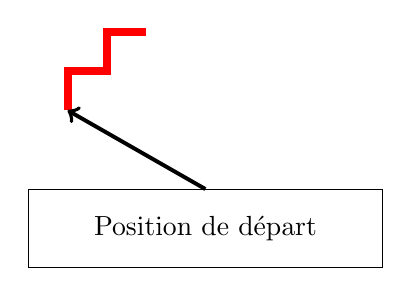
\begin{tikzpicture}[scale=\tikzScale]
            \drawGrid{9}{9}{\gridWidth};       
            \draw[line width= \pathWidth, red ] (1,1) -- (1,2) -- (2,2) -- (2,3) -- (3,3);
            \startRect;
        \end{tikzpicture}&

        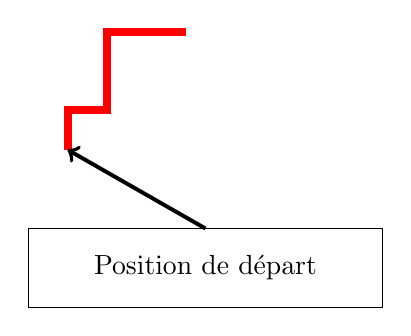
\begin{tikzpicture}[scale=\tikzScale]
            \drawGrid{9}{9}{\gridWidth};
            \draw[line width= \pathWidth, red ] (1,1) -- (1,2) -- (2,2) -- (2,4) -- (4,4);
            \startRect;
        \end{tikzpicture}&

        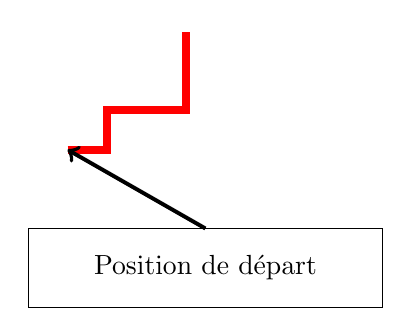
\begin{tikzpicture}[scale=\tikzScale]
            \drawGrid{9}{9}{\gridWidth};
            \draw[line width= \pathWidth, red ] (1,1) -- (2,1) -- (2,2) -- (4,2) -- (4,4);
            \startRect;
        \end{tikzpicture}
    \end{tabularx}
    \end{center}
    
    \item On souhaite maintenant obtenir le motif représenté sur le dessin 4 : 
    


    \begin{center}
        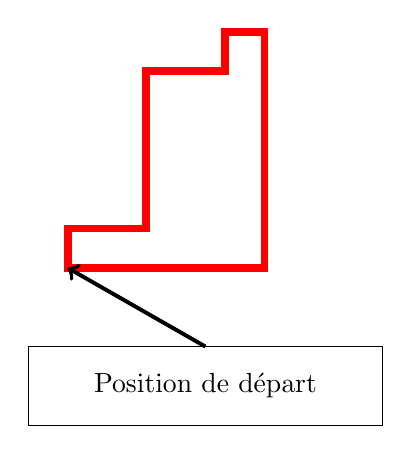
\begin{tikzpicture}[scale=\tikzScale]
            \drawGrid{9}{9}{\gridWidth};
            \draw[line width= \pathWidth, red ] (1,1) -- (1,2) -- (3,2) -- (3,6) -- (5,6) -- (5,7) -- (6,7) -- (6,1) -- cycle;
            \startRect;
        \end{tikzpicture}
    \end{center}
    
    Compléter sans justifier les trois cases du script 3 donné en ANNEXE à rendre avec la copie, 
    permettant d'obtenir le dessin 4.\\

    \item À partir du motif représenté sur le dessin 4, on peut obtenir le pavage ci-dessous :
    
    
    \newcommand{\drawfigure}[4]{
        \draw[line width= \figureWidth, 
        shift={(#1, #2)}, 
        xscale=#3, yscale=#4]
        (0,0) -- (0,1) -- (2,1) -- (2,5) -- (4,5) -- (4,6) -- (5,6) -- (5,0) -- (0,0);
    }

    \newcommand{\writeStr}[3]{
        \node[red, font=\bfseries] at (#2, #3) {#1};
    }

    \begin{center}
        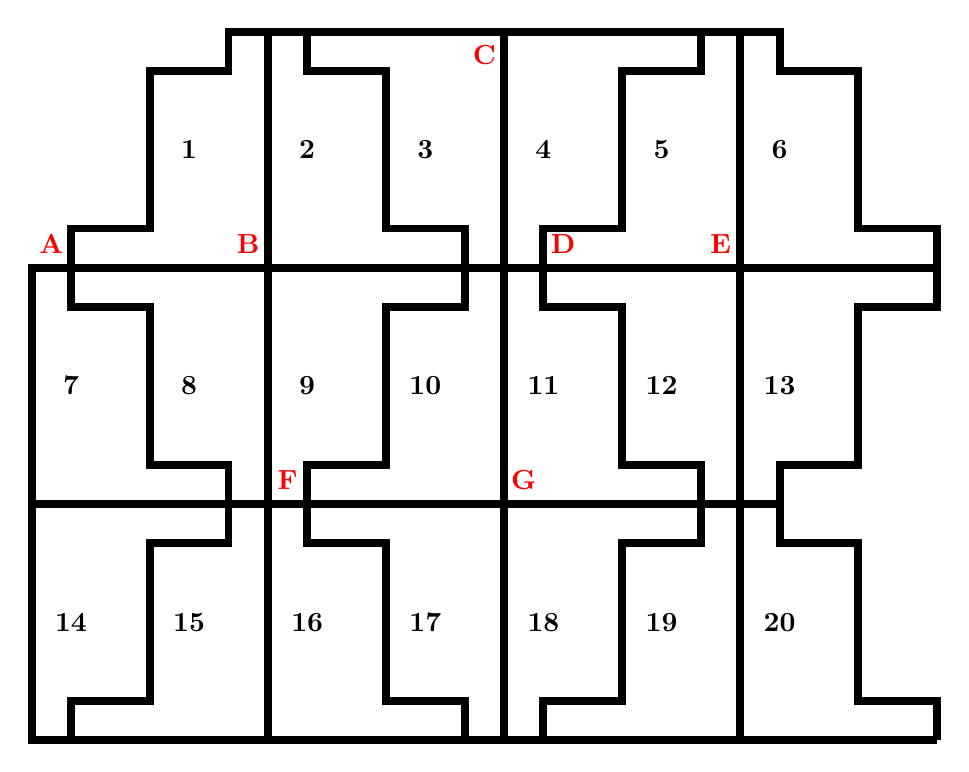
\begin{tikzpicture}[x = 0.5cm, y = 0.5cm]
            \foreach \x/\y/\z/\w in 
            {0/0/1/1, 
            10/0/-1/1, 
            0/0/1/-1, 
            10/0/-1/-1, %
            12/0/1/1, 
            22/0/-1/1, 
            12/0/1/-1, 
            22/0/-1/-1, %
            6/6/1/-1, 
            16/6/-1/-1, %
            6/-6/1/1,
            16/-6/-1/1, 
            6/-6/1/-1,
            16/-6/-1/-1, %
            4/-6/-1/1, 
            4/-6/-1/-1, %
            0/-12/1/1, 
            10/-12/-1/1, %
            12/-12/1/1, 
            22/-12/-1/1}
            {
                \drawfigure{\x}{\y}{\z}{\w};
            }

        \foreach \n in {1,...,21}{
            \ifnum \n=1
            \else
                \pgfmathtruncatemacro{\row}{int((\n - 1) / 7)}
                \pgfmathtruncatemacro{\col}{mod(\n - 1, 7) + 1}
                \pgfmathtruncatemacro{\num}{\n - 1}
                \node[shift={(-3, 3)}, font=\bfseries] at (\col * 3, -\row * 6) {\num};
            \fi
        }
        \foreach \x/\y/\a in 
        {
            -0.5/0.6/A,
            4.5/0.6/B,
            10.5/5.4/C,
            12.5/0.6/D,
            16.5/0.6/E,
            5.5/-5.4/F,
            11.5/-5.4/G,
        }{
            \writeStr{\a}{\x}{\y};
        }
        \end{tikzpicture}
    \end{center}
    
    Répondre aux questions suivantes sur votre copie en indiquant le numéro du motif qui convient (on ne demande pas de justifier la réponse) :
    \begin{enumerate}
        \item Quelle est l'image du motif 1 par la translation qui transforme le point B en E ?
        \item Quelle est l'image du motif 1 par la symétrie de centre B ?
        \item Quelle est l'image du motif 10 par la translation qui transforme le point A en F ?
        \item Quelle est l'image du motif 2 par la symétrie d'axe (CG) ?
    \end{enumerate}	
\end{enumerate}

\newpage
\begin{center}
\textbf{\large ANNEXE à compléter et à rendre avec la copie }
\end{center}

\textbf{Question 1}

\begin{multicols}{2}
    
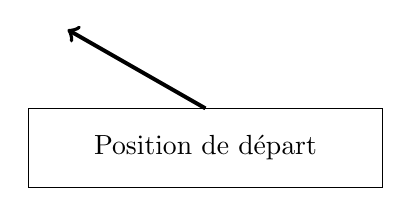
\begin{tikzpicture}[scale=\annexeTikzScale]
    \drawGrid{9}{9}{\gridWidth};
    \startRect;
\end{tikzpicture}

\noindent Chaque côté de carreau mesure 20 pixels.\\
La position de départ du stylo est indiquée sur la figure ci-contre.

\end{multicols}

\textbf{Question 2}

\begin{scratch}[scale=0.8]
    \blockinit{Quand \greenflag est cliqué}
    \blockpen{effacer tout}
    \blockpen{stylo en position d'écriture}
    \blockmove{s'orienter à \ovalnum{0}}
    \blockmove{avancer de \ovalnum{20}}
    \blockmove{tourner \turnright{} de \ovalnum{90} degrés}
    \blockmove{avancer de \ovalnum{\gap*[.]{BLANK}}}
    \blockmove{tourner \turnleft{} de \ovalnum{90} degrés}
    \blockmove{avancer de \ovalnum{80}}
    \blockmove{tourner \turnright{} de \ovalnum{90} degrés}
    \blockmove{avancer de \ovalnum{40}}
    \blockmove{tourner \turnleft{} de \ovalnum{90} degrés}
    \blockmove{avancer de \ovalnum{\gap*[.]{BLANK}}}
    \blockmove{tourner \turnright{} de \ovalnum{90} degrés}
    \blockmove{avancer de \ovalnum{20}}
    \blockmove{tourner \turnright{} de \ovalnum{90} degrés}
    \blockmove{avancer de \ovalnum{\gap*[.]{BLANK}}}
    \blockmove{tourner \turnright{} de \ovalnum{90} degrés}
    \blockmove{avancer de \ovalnum{100}}
\end{scratch}